\documentclass[11pt,a4paper]{article}
\usepackage[margin=25mm]{geometry}
\usepackage{amsmath}
\usepackage{amssymb}
\usepackage{booktabs}
\usepackage{xcolor}
\usepackage[T1]{fontenc}
\usepackage[utf8]{inputenc}
\usepackage{graphicx}
\usepackage[bookmarksdepth=2,colorlinks,linkcolor=blue!50!black,urlcolor=blue!50!black]{hyperref}
\usepackage{tikz}
\usetikzlibrary{arrows.meta,positioning,fit,backgrounds,calc,shapes.misc}
\usepackage{xspace}
\usepackage{multirow}
\usepackage{array}
\usepackage{longtable}
\usepackage{tabularx}
\usepackage{adjustbox}
\usepackage{url}\urlstyle{tt}
\emergencystretch=2em
\usepackage{enumitem}
\setlist{nosep}

% names
\newcommand{\leansmt}{\textsf{lean-smt}\xspace}
\newcommand{\cvcv}{\textsf{cvc5}\xspace}
\newcommand{\verit}{\textsf{veriT}\xspace}
\newcommand{\carcara}{\textsf{Carcara}\xspace}
\newcommand{\alethe}{Alethe\xspace}
\newcommand{\lean}{Lean\xspace}
% code: \detokenize keeps underscores literal inside \texttt
\newcommand{\code}[1]{\texttt{\detokenize{#1}}}
\newcommand{\file}[1]{\texttt{\detokenize{#1}}}
% change classes
\newcommand{\Perf}{\textsf{P}}
\newcommand{\Gen}{\textsf{G}}
\newcommand{\Fix}{\textsf{F}}
\newcommand{\New}{\textsf{N}}
% legend colours, shared by all figures
\definecolor{cNew}{RGB}{220,236,255}      % new, under Smt/Alethe
\definecolor{cNewLib}{RGB}{214,240,214}   % new, placed in the existing tree
\definecolor{cMod}{RGB}{255,236,204}      % existing, modified
\definecolor{cOld}{RGB}{240,240,240}      % existing, untouched
\definecolor{cExt}{RGB}{245,225,245}      % external

\tikzset{
  box/.style={draw, rounded corners=1pt, align=center, font=\small, minimum height=7mm, inner sep=3pt},
  new/.style={box, fill=cNew},
  newlib/.style={box, fill=cNewLib},
  mod/.style={box, fill=cMod},
  old/.style={box, fill=cOld},
  ext/.style={box, fill=cExt},
  arr/.style={-{Latex[length=2mm]}, thick},
  use/.style={-{Latex[length=1.6mm]}, thin, black!60},
  lab/.style={font=\scriptsize, text=black!70},
  grp/.style={draw, dashed, rounded corners, inner sep=4pt},
}

\newcommand{\legend}{%
  \adjustbox{max width=\textwidth}{%
  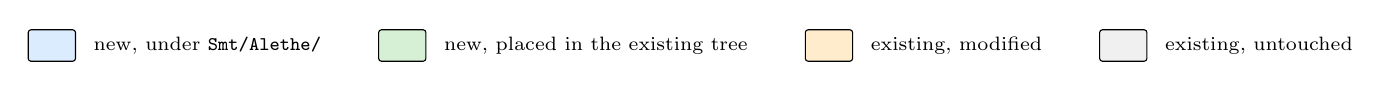
\begin{tikzpicture}[node distance=2mm and 6mm, every node/.style={font=\scriptsize}]
    \node[new, minimum height=4mm, minimum width=6mm, inner sep=1pt] (a) {};
    \node[right=1mm of a] (al) {new, under \file{Smt/Alethe/}};
    \node[newlib, minimum height=4mm, minimum width=6mm, inner sep=1pt, right=of al] (b) {};
    \node[right=1mm of b] (bl) {new, placed in the existing tree};
    \node[mod, minimum height=4mm, minimum width=6mm, inner sep=1pt, right=of bl] (c) {};
    \node[right=1mm of c] (cl) {existing, modified};
    \node[old, minimum height=4mm, minimum width=6mm, inner sep=1pt, right=of cl] (d) {};
    \node[right=1mm of d] (dl) {existing, untouched};
  \end{tikzpicture}}}

\title{The \code{alethe-dev} branch of \leansmt:\\a summary of the changes by code structure}
\author{}
\date{September 2026}

\begin{document}
\maketitle

\begin{abstract}
  The branch \code{alethe-dev} adds an \alethe proof checker to \leansmt, in
  104 commits over the merge base \code{76b4eea} of \code{main}. This note
  describes what was added, organized by code structure rather than by
  chronology: the parser, the changes to the pre-existing library, the new
  verified modules placed inside that library, and the reconstruction of the
  \alethe rules. For each part it gives its size, and for the rule
  reconstruction it lists, rule by rule, which existing \leansmt theorem,
  tactic, verified program or meta-level reconstructor is leveraged.
\end{abstract}

\section{Overview}
\label{sec:overview}

The additions fall into five parts. Three are the ones one expects, namely a
parser for \alethe, the reconstruction of \alethe rules into \lean terms, and
changes to routines that \leansmt already had. Two more are worth separating
out: a set of new \emph{verified} modules that were placed inside the
existing reconstruction tree because both the \cvcv path and the \alethe path
use them, and the driver that checks a proof step by step in the kernel,
which has no counterpart in the tactic-based \cvcv path.
Figure~\ref{fig:pipeline} shows how a proof flows through these parts, and
Table~\ref{tab:sizes} gives their sizes. The pre-existing lemma libraries,
that is every \file{Lemmas.lean}, every \file{Rewrites.lean} and
\file{Prop/Core.lean} under \file{Smt/Reconstruct/}, are byte-identical to
\code{main}.

\begin{figure}[t]
  \centering
  \adjustbox{max width=\textwidth}{%
  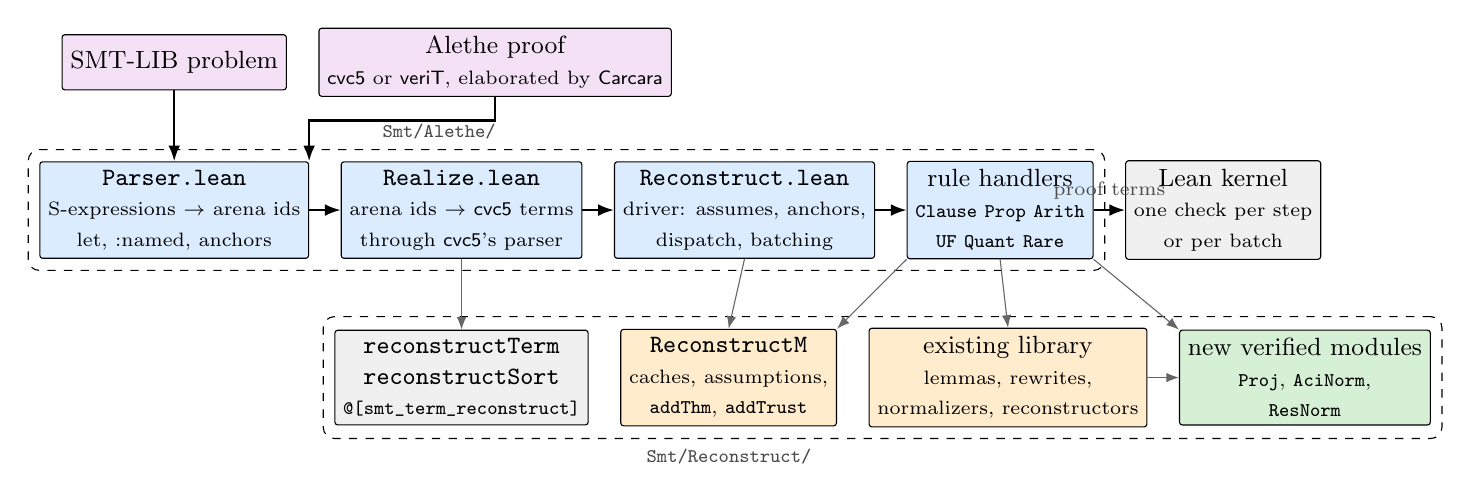
\begin{tikzpicture}[node distance=6mm and 4mm]
    % inputs
    \node[ext] (prob) {SMT-LIB problem};
    \node[ext, right=of prob] (proof) {\alethe proof\\{\scriptsize \cvcv or \verit, elaborated by \carcara}};
    % checker row
    \node[new, below=9mm of prob] (parser) {\file{Parser.lean}\\{\scriptsize S-expressions $\to$ arena ids}\\{\scriptsize let, :named, anchors}};
    \node[new, right=of parser] (realize) {\file{Realize.lean}\\{\scriptsize arena ids $\to$ \cvcv terms}\\{\scriptsize through \cvcv's parser}};
    \node[new, right=of realize] (driver) {\file{Reconstruct.lean}\\{\scriptsize driver: assumes, anchors,}\\{\scriptsize dispatch, batching}};
    \node[new, right=of driver] (rules) {rule handlers\\{\scriptsize \file{Clause} \file{Prop} \file{Arith}}\\{\scriptsize \file{UF} \file{Quant} \file{Rare}}};
    \node[old, right=of rules] (kernel) {\lean kernel\\{\scriptsize one check per step}\\{\scriptsize or per batch}};
    % library row
    \node[old, below=9mm of realize] (term) {\code{reconstructTerm}\\\code{reconstructSort}\\{\scriptsize \code{@[smt_term_reconstruct]}}};
    \node[mod, right=of term] (recm) {\code{ReconstructM}\\{\scriptsize caches, assumptions,}\\{\scriptsize \code{addThm}, \code{addTrust}}};
    \node[mod, right=of recm] (lib) {existing library\\{\scriptsize lemmas, rewrites,}\\{\scriptsize normalizers, reconstructors}};
    \node[newlib, right=of lib] (newlib) {new verified modules\\{\scriptsize \file{Proj}, \file{AciNorm},}\\{\scriptsize \file{ResNorm}}};
    % flow
    \draw[arr] (prob.south) -- (parser.north);
    \draw[arr] (proof.south) -- ++(0,-3mm) -| (parser.north east);
    \draw[arr] (parser) -- (realize);
    \draw[arr] (realize) -- (driver);
    \draw[arr] (driver) -- (rules);
    \draw[arr] (rules) -- node[above, lab] {proof terms} (kernel);
    % uses
    \draw[use] (realize.south) -- (term.north);
    \draw[use] (driver.south) -- (recm.north);
    \draw[use] (rules.south west) -- (recm.north east);
    \draw[use] (rules.south) -- (lib.north);
    \draw[use] (rules.south east) -- (newlib.north west);
    \draw[use] (lib.east) -- (newlib.west);
    \begin{scope}[on background layer]
      \node[grp, fit=(parser)(realize)(driver)(rules), label={[lab]above left:\file{Smt/Alethe/}}] {};
      \node[grp, fit=(term)(recm)(lib)(newlib), label={[lab]below left:\file{Smt/Reconstruct/}}] {};
    \end{scope}
  \end{tikzpicture}}
  \\[2mm]\legend
  \caption{A proof through the checker. The upper row is new; the lower row
    is the pre-existing reconstruction library, which the checker reaches
    through \cvcv's term representation. The realizer hands every term to
    \cvcv's own parser precisely so that the term reconstructors apply
    unchanged.}
  \label{fig:pipeline}
\end{figure}

\begin{table}[t]
  \centering\small
  \begin{tabularx}{\textwidth}{@{}l>{\raggedright\arraybackslash}Xr@{}}
    \toprule
    Part & Files & Lines \\
    \midrule
    \alethe parser & \file{Syntax}, \file{Parser}, \file{Realize} (3 new) & 946 \\
    Rule reconstruction & \file{Basic}, \file{Clause}, \file{Prop}, \file{Arith}, \file{UF}, \file{Quant}, \file{Polyeq}, \file{Lemmas}, \file{Rare}, \file{Rare/Basic} (10 new) & 3\,160 \\
    Generated RARE table & \file{Rare/Rules.lean} (1 new; generator \file{gen.py} 445, input \file{rewrites.eo} 513) & 1\,380 \\
    Driver, frontend, tactic & \file{Reconstruct}, \file{Frontend}, \file{Command}, \file{Tactic}, \file{Alethe.lean} (5 new) & 1\,381 \\
    New verified modules in the existing tree & \file{Prop/AciNorm} 461, \file{Prop/Proj} 239, \file{Prop/ResNorm} 397 (3 new) & 1\,097 \\
    Changes to pre-existing library files & 11 modified & $+1\,361$ / $-791$ \\
    Registration & \file{Smt.lean}, \file{Attribute.lean}, \file{Options.lean} (3 modified) & $+8$ \\
    \midrule
    Tests & \file{Test/Alethe}: 48 test files over 94 problem and proof files & 256 + 15\,037 \\
    Unit tests & \file{Test/Unit/AciNorm}, \file{Test/Unit/ResNorm} (2 new) & 126 \\
    Scripts & \file{check-alethe.sh}, \file{setup-alethe.sh}, \file{rule-boxplots.py} (3 new) & 636 \\
    Report and notes & \file{docs-alethe/}: \TeX{} 1\,246, Markdown 606, plus figures and CSVs & \\
    \bottomrule
  \end{tabularx}
  \caption{Size of each part of the branch. Lines are lines of \lean unless
    stated otherwise. The 104 commits are on top of \code{76b4eea}.}
  \label{tab:sizes}
\end{table}

\section{The parser}
\label{sec:parser}

The parser is self-contained and depends on nothing in the reconstruction
library beyond the S-expression reader \file{Smt/Data/Sexp.lean}, which
existed on \code{main}.

\begin{description}[style=nextline]
\item[\file{Syntax.lean} (205 lines)] The abstract syntax of \alethe proofs,
  parametric in the representation $\tau$ of terms: step arguments
  \code{Arg}, \code{StepData} (id, rule, clause, premises, arguments),
  \code{Command} (assume, step, anchor, subproof) and \code{Proof}. It also
  defines the hash-consed \code{Arena} of S-expression \code{Node}s over
  \code{Nat} ids, with the queries the realizer needs (whether a node is open
  under a binder, its size, its binder variables).
\item[\file{Parser.lean} (508 lines)] Turns the S-expressions of a proof into
  a \code{Proof Nat} over the arena. Every binding construct is eliminated
  here through one environment: parallel \code{let}, \code{:named} (whose
  atoms are computed lazily and once, so that sharing survives), user-level
  \code{define-fun}, and the variable renamings and assignments of
  \code{anchor}. Binders close their variables, so a closed named term is
  resolved once for the whole proof.
\item[\file{Realize.lean} (233 lines)] Turns the \code{Proof Nat} into a
  \code{Proof cvc5.Term}. The SMT-LIB problem and every term of the proof are
  parsed by \cvcv's own parser, through lean-cvc5's \code{InputParser}. Shared
  closed subterms of the arena are sent once, bound with \code{:named}, and
  referred to by name afterwards; open subterms are printed inline. The point
  of this design is that the reconstructor never sees an \alethe-specific
  term: \code{Step.lits} and \code{Premise.lits} are arrays of
  \code{cvc5.Term}, so the whole \code{@[smt_term_reconstruct]} and
  \code{@[smt_sort_reconstruct]} machinery of \leansmt applies unchanged.
\end{description}

\section{Changes to the pre-existing library}
\label{sec:existing}

Eleven files that existed on \code{main} under \file{Smt/Reconstruct/} were
modified, for a net of $+1\,361$ / $-791$ lines. Not all of it is
optimization. Each change is classified below as a performance optimization
of an existing \cvcv routine (\Perf), a generalization so that the \alethe
checker can call an existing routine (\Gen), a bug fix found through the
\alethe evaluation (\Fix), or a new definition (\New).
Figure~\ref{fig:existing} shows where the changes land; the classes are
detailed in the following subsections and summarized in
Table~\ref{tab:existing}.

\begin{figure}[t]
  \centering
  \adjustbox{max width=\textwidth}{%
  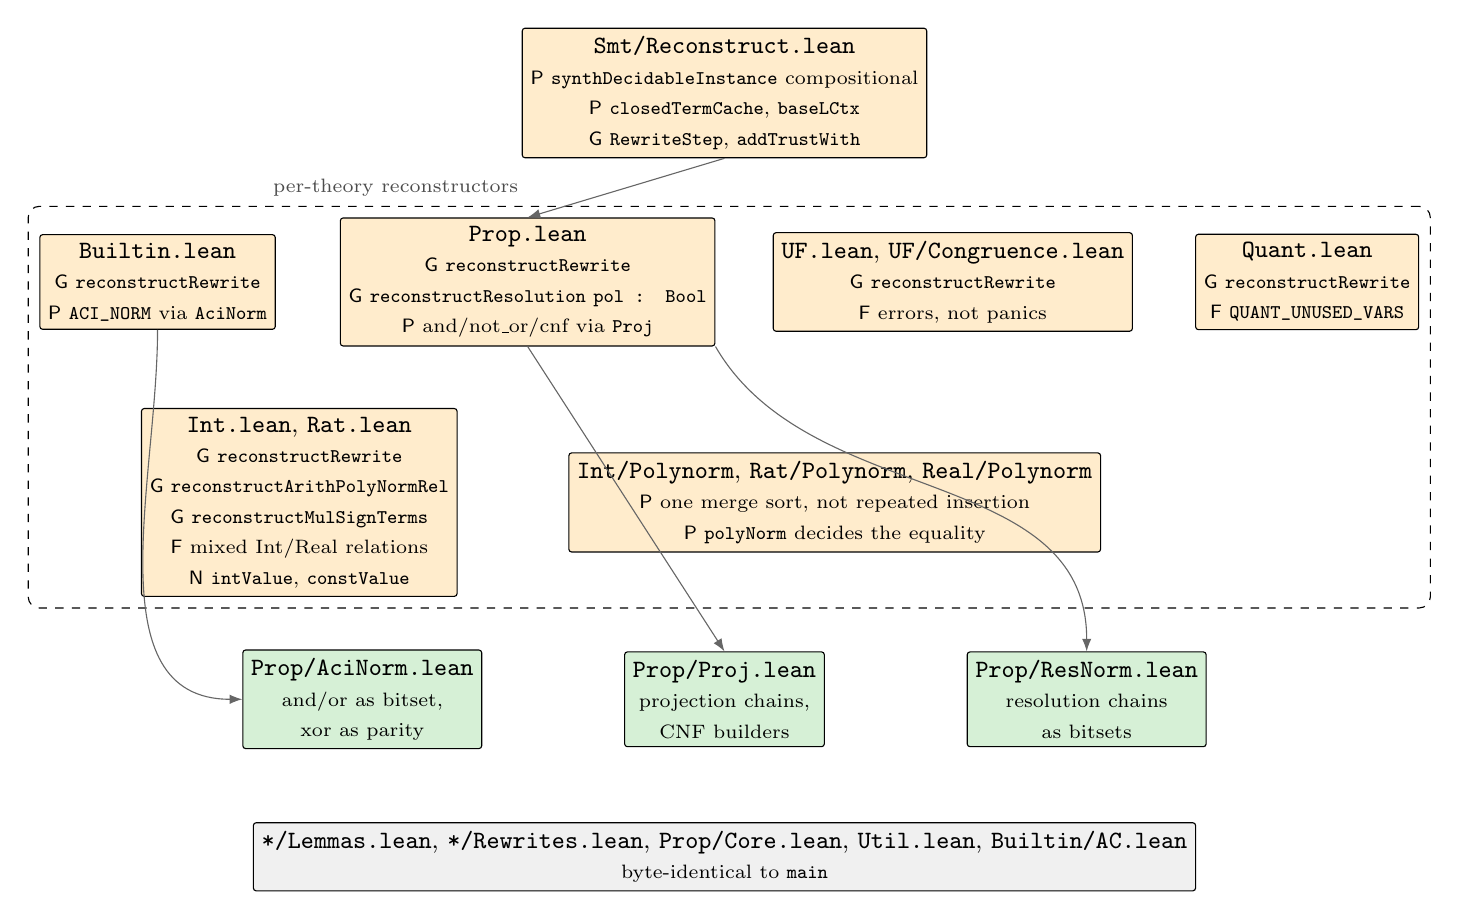
\begin{tikzpicture}[x=1cm, y=1cm]
    % top-level
    \node[mod] (recon) at (0,0) {\file{Smt/Reconstruct.lean}\\{\scriptsize \Perf~\code{synthDecidableInstance} compositional}\\{\scriptsize \Perf~\code{closedTermCache}, \code{baseLCtx}}\\{\scriptsize \Gen~\code{RewriteStep}, \code{addTrustWith}}};
    % per-theory reconstructors
    \node[mod] (builtin) at (-7.2,-2.4) {\file{Builtin.lean}\\{\scriptsize \Gen~\code{reconstructRewrite}}\\{\scriptsize \Perf~\code{ACI_NORM} via \code{AciNorm}}};
    \node[mod] (prop) at (-2.5,-2.4) {\file{Prop.lean}\\{\scriptsize \Gen~\code{reconstructRewrite}}\\{\scriptsize \Gen~\code{reconstructResolution} \code{pol : Bool}}\\{\scriptsize \Perf~and/not\_or/cnf via \code{Proj}}};
    \node[mod] (uf) at (2.9,-2.4) {\file{UF.lean}, \file{UF/Congruence.lean}\\{\scriptsize \Gen~\code{reconstructRewrite}}\\{\scriptsize \Fix~errors, not panics}};
    \node[mod] (quant) at (7.4,-2.4) {\file{Quant.lean}\\{\scriptsize \Gen~\code{reconstructRewrite}}\\{\scriptsize \Fix~\code{QUANT_UNUSED_VARS}}};
    \node[mod] (int) at (-5.4,-5.2) {\file{Int.lean}, \file{Rat.lean}\\{\scriptsize \Gen~\code{reconstructRewrite}}\\{\scriptsize \Gen~\code{reconstructArithPolyNormRel}}\\{\scriptsize \Gen~\code{reconstructMulSignTerms}}\\{\scriptsize \Fix~mixed Int/Real relations}\\{\scriptsize \New~\code{intValue}, \code{constValue}}};
    \node[mod] (poly) at (1.4,-5.2) {\file{Int/Polynorm}, \file{Rat/Polynorm}, \file{Real/Polynorm}\\{\scriptsize \Perf~one merge sort, not repeated insertion}\\{\scriptsize \Perf~\code{polyNorm} decides the equality}};
    % new verified modules
    \node[newlib] (aci) at (-4.6,-7.7) {\file{Prop/AciNorm.lean}\\{\scriptsize and/or as bitset,}\\{\scriptsize xor as parity}};
    \node[newlib] (proj) at (0,-7.7) {\file{Prop/Proj.lean}\\{\scriptsize projection chains,}\\{\scriptsize CNF builders}};
    \node[newlib] (res) at (4.6,-7.7) {\file{Prop/ResNorm.lean}\\{\scriptsize resolution chains}\\{\scriptsize as bitsets}};
    % untouched
    \node[old] (lemmas) at (0,-9.7) {\file{*/Lemmas.lean}, \file{*/Rewrites.lean}, \file{Prop/Core.lean}, \file{Util.lean}, \file{Builtin/AC.lean}\\{\scriptsize byte-identical to \code{main}}};
    % edges
    \draw[use] (recon.south) -- (prop.north);
    \draw[use] (builtin.south) to[out=-90, in=180] (aci.west);
    \draw[use] (prop.south) -- (proj.north);
    \draw[use] (prop.south east) to[out=-60, in=90] (res.north);
    \begin{scope}[on background layer]
      \node[grp, fit=(builtin)(prop)(uf)(quant)(int)(poly), label={[lab]above left:per-theory reconstructors}] {};
    \end{scope}
  \end{tikzpicture}}
  \\[2mm]\legend
  \caption{Where the branch touches the existing reconstruction tree. Every
    per-theory file received the same generalization of its rewrite
    reconstructor; the optimizations concentrate in the polynomial normalizers
    and in \file{Prop.lean}, the latter through the new \file{Proj} module.
    The lemma libraries were not modified.}
  \label{fig:existing}
\end{figure}

\subsection{Performance optimizations (\Perf)}

These change the proof terms the \cvcv path produces, never its conclusions;
each keeps the previous construction as a fallback where one is needed.

\begin{itemize}
\item \textbf{The polynomial normalizer sorts once.} In
  \file{Int/Polynorm.lean}, \file{Rat/Polynorm.lean} and
  \file{Real/Polynorm.lean}, \code{Expr.toPolynomial} used to fold a sum
  through a sorted insertion, so that a sum of $n$ terms cost the kernel
  $O(n^3)$ steps. It now collects the monomials in one pass
  (\code{Expr.flatten}, threading a sign for Int and a rational multiplier
  for Rat and Real so that negation, subtraction and division by a constant
  cost nothing) and sorts them with a bottom-up merge sort
  (\code{mergePairs}, \code{mergeAll}, \code{normalize}), all structurally
  recursive because the kernel does not unfold well-founded recursion. The
  definitions and their denotation lemmas were rewritten and reproved; the
  exported soundness theorem \code{denote_eq_from_toPolynomial_eq} is
  unchanged in statement and proof, and nothing was sorried. Commit
  \code{7258b45}. Measured on a 400-variable sum: 25\,s and 8.9\,GB became
  1.3\,s.
\item \textbf{\code{polyNorm} decides the equality.} The kernel tactic
  closed its goal with \code{Eq.refl} between two normalizer applications,
  which the kernel unifies by unfolding both sides in lockstep instead of
  evaluating each; on large coefficients that ran for over half an hour. It
  now applies \code{of_decide_eq_true} to \code{Eq.refl true}, as
  \code{nativePolyNorm} already did. Meta code only; \code{nativePolyNorm}
  itself is untouched. Commit \code{711e8e7}.
\item \textbf{Projection instead of list indexing.} In \file{Prop.lean}, the
  \cvcv rules \code{AND_ELIM}, \code{NOT_OR_ELIM}, \code{CNF_AND_POS},
  \code{CNF_AND_NEG}, \code{CNF_OR_POS} and \code{CNF_OR_NEG} projected the
  $i$-th conjunct through \code{andN} and \code{List.getElem} with a decided
  bound, charging every step for the whole conjunction. They now walk the
  right-nested \code{And} the hypothesis already is, through the new
  \file{Prop/Proj.lean} (Section~\ref{sec:newlib}). \code{CNF_OR_POS}
  collapses to the single node \code{notOrSelf}. Commit \code{008ac35}.
\item \textbf{\code{ACI_NORM} through the reflective normalizer.} In
  \file{Builtin.lean}, an and/or layer is normalized by the verified
  \code{AciNorm} normalizer, evaluated by the kernel; other operators and any
  failure fall back to the previous AC rewriting tactic. Kernel time for a
  200-atom layer drops from seconds to about 30\,ms. Commit \code{28bb705}.
\item \textbf{Decidable instances and closed-term caching.} In
  \file{Smt/Reconstruct.lean}, \code{synthDecidableInstance} guards the
  instance search (whose own ``failed to synthesize'' used to escape and take
  down whole runs on QF\_UFIDL) and, when the search fails, builds the
  instance compositionally through $\neg$, $\wedge$, $\vee$ and
  $\leftrightarrow$ so that it matches the instance a theorem over
  \code{[Decidable c]} elaborates to. The reconstruction state gains a
  \code{closedTermCache}, valid across binder scopes, enabled only when a
  driver sets \code{baseLCtx}; the \cvcv path leaves it off.
\end{itemize}

\subsection{Generalizations for sharing (\Gen)}

Pure refactors with no behavior change on the \cvcv path, almost all in the
first commit \code{c69e4d5}.

\begin{itemize}
\item A record \code{RewriteStep} (rule, arguments, list arguments, result,
  lazily reconstructed premises) in \file{Smt/Reconstruct.lean} decouples a
  rewrite step from \code{cvc5.Proof}. Every per-theory
  \code{reconstructRewrite} in \file{Builtin}, \file{Int}, \file{Prop},
  \file{Quant}, \file{Rat} and \file{UF} was retyped to take it, and each
  \cvcv call site wraps its proof with \code{RewriteStep.ofProof}. This is
  what lets an \alethe \code{rare_rewrite} or \code{qnt_join} step, which has
  no proof object, reach the existing rewrite reconstructors.
\item \code{Prop.getResolutionResult} and \code{Prop.reconstructResolution}
  take the pivot polarity as a \code{Bool} rather than a \cvcv term;
  \code{Prop.isNotOf} became public.
\item In \file{Int.lean} and \file{Rat.lean}, \code{reconstructArithPolyNormRel}
  takes the premise's term and proof instead of a proof object, and the
  term-level half of the mult-sign reconstruction was factored out as
  \code{reconstructMulSignTerms}, the old name staying as a two-line wrapper
  (commit \code{eab472d}).
\item \code{addTrustWith} lets a step be trusted with a custom trace message.
\end{itemize}

\subsection{Bug fixes (\Fix)}

\begin{itemize}
\item \file{Quant.lean}: \code{QUANT_UNUSED_VARS} was wrong when a prefix
  binds the same variable twice or reorders (\cvcv reuses the variable node
  for a name, and the body refers to the innermost binder), and again when
  every binder is dropped and the body is itself a quantifier. Each side is
  now instantiated from the binders of the other. Commits \code{3ca2f21},
  \code{4d88b28}. A regression test with a repeated binder was added.
\item \file{Int.lean}, \file{Rat.lean}: a relation with one Int side and one
  Real side was claimed by the Int handler and reconstructed ill-sorted. The
  Int handler now declines unless both sides are integer, and the Rat handler
  casts through a new \code{ratArg} helper.
\item \file{UF/Congruence.lean}: the left- and right-associative congruence
  helpers replaced panicking \code{Option.get!} and \code{hs[0]!} with
  errors, so a premise that is not an equality is reported instead of
  becoming a dummy term the kernel then rejects. Commit \code{ad066ae}.
\end{itemize}

\subsection{New definitions (\New)}

\code{Int.intValue} and \code{Rat.constValue} read a coefficient written as
\alethe writes it, as a negated literal \code{(- 1)} or a quotient of
literals \code{(/ 1 4)}; for \cvcv input they agree with the previous
direct reads. No new theorem was added to any pre-existing file.

\begin{table}[t]
  \centering\small
  \begin{tabular}{@{}lrrl@{}}
    \toprule
    File & $+$ & $-$ & Classes \\
    \midrule
    \file{Smt/Reconstruct.lean} & 97 & 10 & \Perf~\Gen \\
    \file{Builtin.lean} & 50 & 40 & \Gen~\Perf \\
    \file{Int.lean} & 114 & 97 & \Gen~\Fix~\New \\
    \file{Int/Polynorm.lean} & 222 & 92 & \Perf \\
    \file{Prop.lean} & 134 & 142 & \Gen~\Perf \\
    \file{Quant.lean} & 67 & 54 & \Gen~\Fix \\
    \file{Rat.lean} & 121 & 86 & \Gen~\Fix~\New \\
    \file{Rat/Polynorm.lean} & 256 & 120 & \Perf \\
    \file{Real/Polynorm.lean} & 263 & 121 & \Perf \\
    \file{UF.lean} & 21 & 21 & \Gen \\
    \file{UF/Congruence.lean} & 16 & 8 & \Fix \\
    \bottomrule
  \end{tabular}
  \caption{The modified pre-existing files under \file{Smt/Reconstruct/}
    and the classes of change each received.}
  \label{tab:existing}
\end{table}

\section{New verified modules in the existing tree}
\label{sec:newlib}

Three modules were added under \file{Smt/Reconstruct/Prop/} rather than
under \file{Smt/Alethe/}, because they are reflective checkers in the style
of the polynomial normalizer and serve both paths. Each has a verified core
of ordinary definitions and theorems, and a small meta layer that reifies an
expression and applies the soundness theorem as a term.

\begin{description}[style=nextline]
\item[\file{Prop/Proj.lean} (239 lines, 8 theorems)] Projection out of a
  right-nested $\wedge$ or $\neg\vee$ chain, and the builders of the CNF
  axioms (\code{mkAndProj}, \code{mkNotOrProj}, \code{mkOrInj},
  \code{mkCnfAndPos}, \code{mkCnfAndNeg}, \code{mkCnfOrNeg},
  \code{notOrSelf}). A \code{ProjChain} keeps the partially unrolled spine
  so that a step projecting many indices out of one hypothesis builds $O(n)$
  nodes in total. Used by the \cvcv rules named above and by the \alethe
  rules \code{and}, \code{not_or}, \code{and_pos}, \code{and_neg},
  \code{or_pos}, \code{or_neg}, \code{onepoint} and \code{distinct_elim}.
\item[\file{Prop/AciNorm.lean} (461 lines, 20 theorems)] One layer of
  $\wedge$ or $\vee$ is reified into a tree over indexed atoms and normalized
  to a bitset, \code{none} when the annihilator occurs; a layer of xor is
  normalized to the parity of its atoms. The kernel evaluates the normal
  form with its accelerated \code{Nat} bit operations. Used by \cvcv's
  \code{ACI_NORM} and by \alethe's \code{semilattice_simp} and
  \code{boolean_group_simp}.
\item[\file{Prop/ResNorm.lean} (397 lines, 18 theorems)] A checker for
  resolution chains and the containment rules. A literal is a \code{Nat}, a
  clause is both a \code{List Nat} whose denotation unfolds definitionally to
  the stated proposition and a bitset on which each link of a chain is a few
  accelerated operations; the pivots are hints, so a wrong one fails only at
  the final containment. It depends on \code{propext} and \code{Quot.sound}
  only. Used by the \alethe clausal rules behind the option
  \code{smt.alethe.reflect}, default off; the \cvcv path does not use it
  yet.
\end{description}

\section{Reconstruction of the \alethe rules}
\label{sec:rules}

The rule handlers are registered with a new attribute
\code{alethe_rule_reconstruct}, added to the existing attribute framework in
three lines of \file{Smt/Attribute.lean} and collected by the existing
\code{getReconstructors}. Five handlers cover the rules, one per family
(\file{Clause}, \file{Prop}, \file{Arith}, \file{UF}, \file{Quant}), with
\file{Rare} dispatched from \file{UF}.

This section covers the rules that reach the checker after \carcara's
pipeline as the evaluation runs it: \code{polyeq}, \code{local},
\code{core-simp-rare} restricted by \code{--core-rules} to the
\code{*_simplify} family and the legacy \code{ac_simp}, \code{aci_simp} and
\code{absorb}, \code{budget}, and the \code{reordering} pass. Those passes
remove the \code{*_simplify} rules and the legacy ACI rules (replaced by
\code{rare_rewrite} and \code{evaluate} chains and by the structural
\code{semilattice_simp}, \code{boolean_group_simp} and \code{assoc_simp})
and \code{reordering}. The non-linear multiplication rules are left out as
well. The handlers also accept those rules, so that a raw solver proof can
be checked, but they are not covered here. The reconstructors of
\code{bfun_elim}, \code{th_resolution} and \code{strict_resolution} have
been dropped, no corpus of the evaluation emitting them after the pipeline.
Figure~\ref{fig:rules} shows which existing component each family draws on;
the subsections list every rule. Throughout, a component is \emph{existing}
if it is present on \code{main} and \emph{new} otherwise; the new verified
modules of Section~\ref{sec:newlib} are marked as such.

\begin{figure}[t]
  \centering
  \adjustbox{max width=\textwidth}{%
  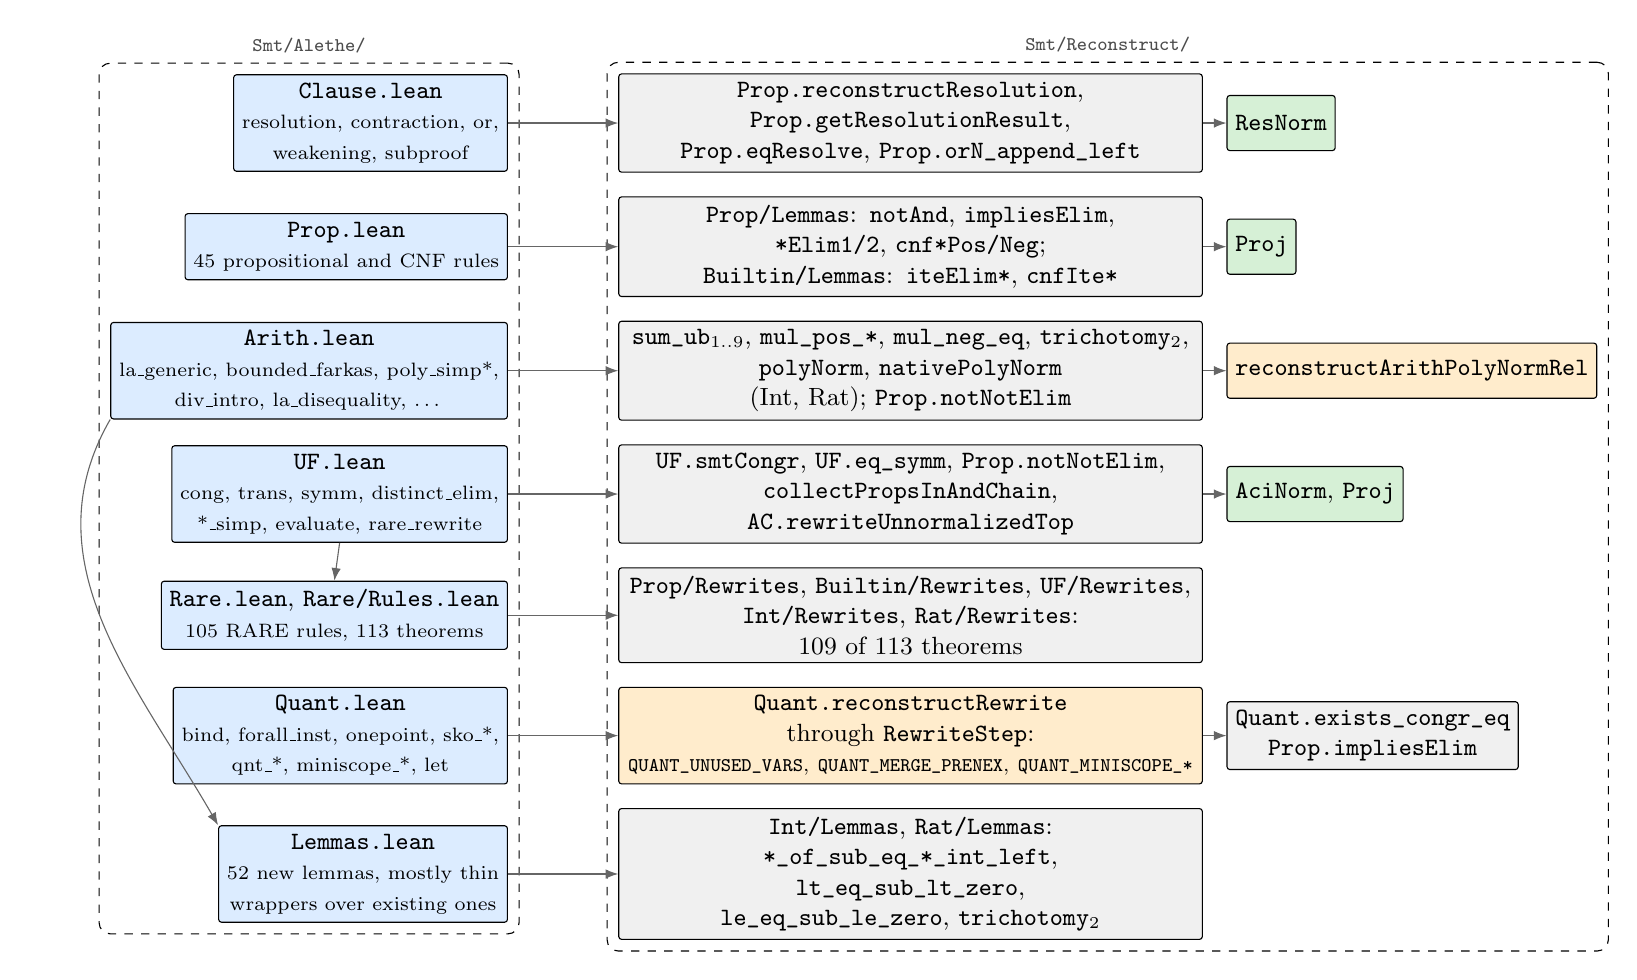
\begin{tikzpicture}[node distance=3mm and 3mm, rc/.style={old, text width=72mm}]
    % right column: existing components, chained vertically
    \node[rc] (resol) {\code{Prop.reconstructResolution}, \code{Prop.getResolutionResult},\\\code{Prop.eqResolve}, \code{Prop.orN_append_left}};
    \node[rc, below=of resol] (proplem) {\file{Prop/Lemmas}: \code{notAnd}, \code{impliesElim}, \code{*Elim1/2}, \code{cnf*Pos/Neg};\\\file{Builtin/Lemmas}: \code{iteElim*}, \code{cnfIte*}};
    \node[rc, below=of proplem] (arithlem) {\code{sum_ub}$_{1..9}$, \code{mul_pos_*}, \code{mul_neg_eq}, \code{trichotomy}$_2$,\\\code{polyNorm}, \code{nativePolyNorm} (Int, Rat); \code{Prop.notNotElim}};
    \node[rc, below=of arithlem] (uflem) {\code{UF.smtCongr}, \code{UF.eq_symm}, \code{Prop.notNotElim},\\\code{collectPropsInAndChain}, \code{AC.rewriteUnnormalizedTop}};
    \node[rc, below=of uflem] (rewrites) {\file{Prop/Rewrites}, \file{Builtin/Rewrites}, \file{UF/Rewrites},\\\file{Int/Rewrites}, \file{Rat/Rewrites}: 109 of 113 theorems};
    \node[mod, text width=72mm, below=of rewrites] (quantrw) {\code{Quant.reconstructRewrite} through \code{RewriteStep}:\\{\scriptsize \code{QUANT_UNUSED_VARS}, \code{QUANT_MERGE_PRENEX}, \code{QUANT_MINISCOPE_*}}};
    \node[rc, below=of quantrw] (base) {\file{Int/Lemmas}, \file{Rat/Lemmas}: \code{*_of_sub_eq_*_int_left},\\\code{lt_eq_sub_lt_zero}, \code{le_eq_sub_le_zero}, \code{trichotomy}$_2$};
    % side boxes
    \node[newlib, right=of resol] (resnorm) {\code{ResNorm}};
    \node[newlib, right=of proplem] (proj) {\code{Proj}};
    \node[mod, right=of arithlem] (arithmeta) {\code{reconstructArithPolyNormRel}};
    \node[newlib, right=of uflem] (aci) {\code{AciNorm}, \code{Proj}};
    \node[old, right=of quantrw] (quantlem) {\code{Quant.exists_congr_eq}\\\code{Prop.impliesElim}};
    % left column: handler families
    \node[new, left=14mm of resol] (clause) {\file{Clause.lean}\\{\scriptsize resolution, contraction, or,}\\{\scriptsize weakening, subproof}};
    \node[new, left=14mm of proplem] (prop) {\file{Prop.lean}\\{\scriptsize 45 propositional and CNF rules}};
    \node[new, left=14mm of arithlem] (arith) {\file{Arith.lean}\\{\scriptsize la\_generic, bounded\_farkas, poly\_simp*,}\\{\scriptsize div\_intro, la\_disequality, \ldots}};
    \node[new, left=14mm of uflem] (uf) {\file{UF.lean}\\{\scriptsize cong, trans, symm, distinct\_elim,}\\{\scriptsize *\_simp, evaluate, rare\_rewrite}};
    \node[new, left=14mm of rewrites] (rare) {\file{Rare.lean}, \file{Rare/Rules.lean}\\{\scriptsize 105 RARE rules, 113 theorems}};
    \node[new, left=14mm of quantrw] (quant) {\file{Quant.lean}\\{\scriptsize bind, forall\_inst, onepoint, sko\_*,}\\{\scriptsize qnt\_*, miniscope\_*, let}};
    \node[new, left=14mm of base] (lemmas) {\file{Lemmas.lean}\\{\scriptsize 52 new lemmas, mostly thin}\\{\scriptsize wrappers over existing ones}};
    % edges
    \foreach \a/\b in {clause/resol, prop/proplem, arith/arithlem, uf/uflem, rare/rewrites, quant/quantrw, lemmas/base}
      \draw[use] (\a.east) -- (\b.west);
    \foreach \a/\b in {resol/resnorm, proplem/proj, arithlem/arithmeta, uflem/aci, quantrw/quantlem}
      \draw[use] (\a.east) -- (\b.west);
    \draw[use] (uf.south) -- (rare.north);
    \draw[use] (arith.south west) to[out=-120, in=120] (lemmas.north west);
    \begin{scope}[on background layer]
      \node[grp, fit=(clause)(prop)(arith)(uf)(rare)(quant)(lemmas), label={[lab]above:\file{Smt/Alethe/}}] {};
      \node[grp, fit=(resol)(resnorm)(proplem)(proj)(arithlem)(arithmeta)(uflem)(aci)(rewrites)(quantrw)(quantlem)(base), label={[lab]above:\file{Smt/Reconstruct/}}] {};
    \end{scope}
  \end{tikzpicture}}
  \\[2mm]\legend
  \caption{What each rule family leverages. Grey boxes are components that
    existed on \code{main} and were not modified; orange ones existed and
    were generalized or factored out on the branch; green ones are the new
    verified modules of Section~\ref{sec:newlib}.}
  \label{fig:rules}
\end{figure}

\subsection{Substrate shared by every rule}

Before any rule, the checker reuses the reconstruction monad and its
services unchanged: \path{ReconstructM} with \path{Reconstruct.Context} and
\path{Reconstruct.State}; the term and proof caches, \path{withNewTermCache}
and \path{withNewProofCache}; the assumption handling, \path{withAssums} and
\path{findAssumWithType?}; the step recorders
\path{addThm}, \path{addTac} and \path{addTrust}, and the option
\path{useNative}. Terms and sorts go through \path{reconstructTerm},
\path{reconstructSort} and \path{reconstructSortLevelAndSort}, hence through
every \path{@[smt_term_reconstruct]} and \path{@[smt_sort_reconstruct]}
handler of \path{Prop}, \path{Builtin}, \path{UF}, \path{Int}, \path{Rat},
\path{Real}, \path{BitVec} and \path{Datatype}. The \path{alethe} tactic
reuses the entire \path{smt} front end: \path{Preprocess.mono},
\path{pushHintsToCtx}, \path{intros}, \path{negateGoal}, \path{normalize},
\path{embedding}, \path{applySteps}, \path{genUniqueFVarNames},
\path{prepareSmtQuery}, \path{Command.cmdsAsQuery} and the
\path{Config}/\path{Result} types. The problem's symbols are introduced with
\path{reconstructSort} through a flat \path{withLocalDecls} rather than one
nested \path{withLocalDecl} per declaration, and \path{choice} symbols are
bound to \path{Classical.epsilon} over \path{reconstructSortLevelAndSort}.

\subsection{Clausal rules (\file{Clause.lean}, 227 lines)}

\begin{center}\footnotesize
\begin{tabularx}{\textwidth}{@{}l>{\raggedright\arraybackslash}X@{}}
  \toprule
  Rule & Component \\
  \midrule
  \code{resolution} & existing \code{Prop.reconstructResolution}, \code{Prop.getResolutionResult}; \\
  & new \code{ResNorm.proveClause} when \code{smt.alethe.reflect} is set \\
  \code{contraction}, \code{or} & new lemma \code{orN_of_map}; \code{ResNorm} when set \\
  \code{weakening} & existing \code{Prop.orN_append_left} \\
  \code{subproof} & new lemma \code{orN_of_impliesN} \\
  \code{hole} & trusted, through \code{addTrustWith} \\
  \bottomrule
\end{tabularx}
\end{center}

The fix-up that reconciles a computed clause with the stated one
(permutations, duplicates, flattening) uses the existing \path{Prop.eqResolve}
and the existing AC tactic \path{Meta.AC.rewriteUnnormalizedTop} from
\path{Builtin/AC.lean} as its last resort. Resolution on a premise that
itself holds the pivot no longer re-resolves. The existing resolution
reconstructor is the largest single reuse in the checker.

\subsection{Propositional rules (\file{Prop.lean}, 266 lines)}

Of the 45 rules, 40 are direct applications of lemmas that existed in
\file{Prop/Lemmas.lean} and \file{Builtin/Lemmas.lean}.

\begin{center}\footnotesize
\begin{tabularx}{\textwidth}{@{}l>{\raggedright\arraybackslash}X@{}}
  \toprule
  Rule & Component \\
  \midrule
  \code{not_and} & existing \code{Prop.notAnd} \\
  \code{implies} & existing \code{Prop.impliesElim} \\
  \code{not_implies1}, \code{not_implies2} & existing \code{Prop.notImplies1}, \code{Prop.notImplies2} \\
  \code{equiv1}, \code{equiv2} & existing \code{Prop.equivElim1}, \code{Prop.equivElim2} \\
  \code{not_equiv1}, \code{not_equiv2} & existing \code{Prop.notEquivElim1}, \code{Prop.notEquivElim2} \\
  \code{xor1}, \code{xor2} & existing \code{Prop.xorElim1}, \code{Prop.xorElim2} \\
  \code{not_xor1}, \code{not_xor2} & existing \code{Prop.notXorElim1}, \code{Prop.notXorElim2} \\
  \code{ite1}, \code{ite2} & existing \code{Builtin.iteElim2}, \code{Builtin.iteElim1} \\
  \code{not_ite1}, \code{not_ite2} & existing \code{Builtin.notIteElim2}, \code{Builtin.notIteElim1} \\
  \code{implies_pos} & existing \code{Prop.cnfImpliesPos} \\
  \code{implies_neg1}, \code{implies_neg2} & existing \code{Prop.cnfImpliesNeg1}, \code{Prop.cnfImpliesNeg2} \\
  \code{equiv_pos1}, \code{equiv_pos2} & existing \code{Prop.cnfEquivPos2}, \code{Prop.cnfEquivPos1} \\
  \code{equiv_neg1}, \code{equiv_neg2} & existing \code{Prop.cnfEquivNeg2}, \code{Prop.cnfEquivNeg1} \\
  \code{xor_pos1}, \code{xor_pos2} & existing \code{Prop.cnfXorPos1}, \code{Prop.cnfXorPos2} \\
  \code{xor_neg1}, \code{xor_neg2} & existing \code{Prop.cnfXorNeg2}, \code{Prop.cnfXorNeg1} \\
  \code{ite_pos1}, \code{ite_pos2} & existing \code{Builtin.cnfItePos2}, \code{Builtin.cnfItePos1} \\
  \code{ite_neg1}, \code{ite_neg2} & existing \code{Builtin.cnfIteNeg2}, \code{Builtin.cnfIteNeg1} \\
  \code{and}, \code{not_or} & new \code{Proj.mkAndProj}, \code{Proj.mkNotOrProj} \\
  \code{and_pos}, \code{and_neg}, \code{or_neg} & new \code{Proj.mkCnfAndPos}, \code{mkCnfAndNeg}, \code{mkCnfOrNeg} \\
  \code{or_pos} & new \code{Proj.notOrSelf} \\
  \code{true} & \code{trivial} \\
  \code{false}, \code{not_not} & new lemmas \code{not_false_cl}, \code{not_not_cl} \\
  \code{ite_then_intro}, \code{ite_else_intro} & new lemmas of the same names \\
  \code{connective_def}, \code{qnt_duality} & new lemmas \code{connective_def_xor/eq/ite}; quantifier cases by a small \code{simp} set; existing \code{synthDecidableInstance} \\
  \code{and_intro} & new meta code, an \code{And.intro} fold \\
  \bottomrule
\end{tabularx}
\end{center}

\subsection{Arithmetic rules (\file{Arith.lean}, 553 lines)}

The Farkas driver behind \code{la_generic}, \code{la_tautology} and
\code{bounded_farkas} is new meta code, about 340 lines: the negations of the clause's literals are
assumed, oriented into bounds, strengthened for strict integer bounds,
scaled by the coefficients given as \code{:args}, summed, and refuted
through the normalized difference of the two sides and a decidable fact
about the resulting constant. Every proof-level ingredient of that driver is
existing.

\begin{center}\footnotesize
\begin{tabularx}{\textwidth}{@{}l>{\raggedright\arraybackslash}X@{}}
  \toprule
  Rule & Component \\
  \midrule
  \code{la_generic}, \code{la_tautology}, \code{bounded_farkas} & existing \code{Int.sum_ub}$_{1..9}$, \code{Rat.sum_ub}$_{1..9}$; existing \code{mul_pos_lt/le/eq}, \code{mul_neg_eq} (Int, Rat); existing \code{Int.polyNorm}, \code{Rat.polyNorm} and their native variants; existing \code{Prop.notNotElim}; \lean core \code{omega} for integer tightening; new lemmas \code{farkas_lt/le/eq} (Int, Rat), \code{orN_of_impliesN_not} \\
  \code{poly_simp} & existing \code{Int.polyNorm}, \code{Rat.polyNorm}, and native variants \\
  \code{poly_simp_rel} & \code{reconstructArithPolyNormRel} (Int, Rat), generalized from the existing handler; nine new mixed-sort lemmas over the existing \code{Rat.*_of_sub_eq_*_int_left} \\
  \code{la_rw_eq} & new lemmas \code{Int.la_rw_eq}, \code{Rat.la_rw_eq} over existing \code{Rat.trichotomy}$_2$ \\
  \code{la_disequality} & new lemmas over existing \code{Rat.trichotomy}$_2$ \\
  \code{la_totality} & new lemmas \code{Int.la_totality}, \code{Rat.la_totality} \\
  \code{div_intro} & new lemmas \code{div_intro_pos/neg/real}; \code{omega} for a constant divisor \\
  \code{div_by_zero_intro} & new lemma \code{div_by_zero_intro} \\
  \code{lia_generic} & \lean core \code{omega} only; a step outside its fragment is trusted \\
  \bottomrule
\end{tabularx}
\end{center}

The new Farkas, disequality, totality and \path{la_rw_eq} lemmas in
\path{Alethe/Lemmas.lean} are themselves proved from existing
\path{Rat.trichotomy}$_2$, \path{Rat.lt_eq_sub_lt_zero}, \path{Rat.le_eq_sub_le_zero},
\path{Rat.lt_of_le_of_lt}, \path{Rat.lt_of_lt_of_le} and \path{Rat.le_of_lt}.
No \leansmt tactic is invoked by name: the polynomial normalizer is called
as a function on a goal, and \path{omega} is \lean's.

\subsection{Equality and rewriting rules (\file{UF.lean}, 556 lines)}

\begin{center}\footnotesize
\begin{tabularx}{\textwidth}{@{}l>{\raggedright\arraybackslash}X@{}}
  \toprule
  Rule & Component \\
  \midrule
  \code{cong} & existing \code{UF.smtCongr}, \code{UF.eq_symm}; new \code{transportEq} for \code{distinct} \\
  \code{eq_congruent}, \code{eq_congruent_pred} & existing \code{UF.smtCongr}, \code{Prop.notNotElim}; new lemma \code{orN_of_impliesN_not} \\
  \code{eq_transitive} & existing \code{Prop.notNotElim}; new chaining over \code{Eq.trans} \\
  \code{eq_symmetric} & existing \code{UF.eq_symm}, \code{Prop.impliesElim} \\
  \code{refl}, \code{eq_reflexive} & existing \code{reconstructSortLevelAndSort} \\
  \code{symm}, \code{not_symm}, \code{trans} & new meta code over \code{Eq.symm}, \code{Ne.symm}, \code{Eq.trans}, with defeq-aware orientation under anchor \code{let}s \\
  \code{distinct_elim} & existing \code{collectPropsInAndChain}; new \code{Proj.ProjChain}; new lemmas \code{ne_symm_eq}, \code{distinct_bool_false} \\
  \code{semilattice_simp} & new \code{AciNorm.proveEq} \\
  \code{boolean_group_simp} & new \code{AciNorm.proveXorEq} \\
  \code{assoc_simp} & existing \code{Meta.AC.rewriteUnnormalizedTop} \\
  \code{evaluate} & existing \code{synthDecidableInstance}; new \code{decideProofOfNative}, \code{proveByCases}, \code{decideGround} \\
  \code{rare_rewrite} & dispatched to \file{Rare.lean}, below \\
  \bottomrule
\end{tabularx}
\end{center}

\subsection{RARE rewrites (\file{Rare.lean} 109, \file{Rare/Basic.lean} 44, \file{Rare/Rules.lean} 1\,380 lines)}

A \code{rare_rewrite} step names a rule of the RARE file \carcara was run
with; the \code{core-simp-rare} pass replays every \code{*_simplify} step as
a chain of such steps and \code{evaluate}. The generator \file{gen.py} reads
that file, \file{rewrites.eo}, and emits one theorem per rule, two for rules
polymorphic over Int and Real, plus a dispatch table describing each rule's
arguments; existing proofs are preserved across regenerations.
\file{Rare.lean} instantiates the theorem with the step's arguments by a
reducing telescope and unification.

Leaving aside the two non-linear \code{mult-tangent} rules, the table holds
105 rules and 113 theorems. Their proofs are almost entirely existing
lemmas:

\begin{center}\footnotesize
\begin{tabularx}{\textwidth}{@{}>{\raggedright\arraybackslash}Xr@{}}
  \toprule
  Proof of the generated theorem & Theorems \\
  \midrule
  existing \code{Int.Rewrite.*} and \code{Rat.Rewrite.*} lemmas (\file{Int/Rewrites}, \file{Rat/Rewrites}) & 45 \\
  existing \code{Prop.bool_*} and \code{Prop.ite_*} lemmas (\file{Prop/Rewrites}) & 41 \\
  existing \code{Builtin.ite_*} and \code{UF.eq_*}, \code{UF.distinct_binary_elim} (\file{Builtin/Rewrites}, \file{UF/Rewrites}) & 13 \\
  \code{rfl} & 8 \\
  \lean core \code{Int.emod_emod}, \code{Int.emod_def}, or an inline \code{propext} & 3 \\
  short tactic proof & 2 \\
  new lemma \code{or_not_refl} (a rule newer than lean-cvc5's enumeration) & 1 \\
  \bottomrule
\end{tabularx}
\end{center}

Six \code{array-*} rules have no statement, there being no array sort
support, and are trusted. The rule \code{distinct-false} is special-cased in
\file{UF.lean} through \code{Proj.mkAndProj}.

\subsection{Quantifier rules (\file{Quant.lean}, 655 lines)}

\begin{center}\footnotesize
\begin{tabularx}{\textwidth}{@{}l>{\raggedright\arraybackslash}X@{}}
  \toprule
  Rule & Component \\
  \midrule
  \code{qnt_rm_unused} ($\forall$) & existing \code{Quant.reconstructRewrite} at \code{QUANT_UNUSED_VARS} \\
  \code{qnt_join} & existing \code{Quant.reconstructRewrite} at \code{QUANT_MERGE_PRENEX} \\
  \code{miniscope_distribute} & existing \code{Quant.reconstructRewrite} at \code{QUANT_MINISCOPE_AND} \\
  \code{miniscope_split} & existing \code{Quant.reconstructRewrite} at \code{QUANT_MINISCOPE_OR} \\
  \code{miniscope_ite} & existing \code{Quant.reconstructRewrite} at \code{QUANT_MINISCOPE_ITE} \\
  \code{forall_inst} & existing \code{Prop.impliesElim}; new \code{alignInstances} \\
  \code{bind} & existing \code{Quant.exists_congr_eq}, \lean core \code{forall_congr}; new lemma \code{orN_forall} \\
  \code{onepoint} & new \code{Proj.mkOrInj}, \code{Proj.mkAndProj}; existing \code{collectPropsInOrChain}, \code{collectPropsInAndChain}; new lemmas \code{onepoint_forall}, \code{onepoint_exists} \\
  \code{sko_ex}, \code{sko_forall} & new lemmas \code{sko_ex_eq}, \code{sko_forall_eq} \\
  \code{qnt_simplify} & new lemmas \code{qnt_forall_true/false}, \code{qnt_exists_true/false} \\
  \code{let} & new meta code, a \code{mkCongrArg} chain over anchor \code{let}s \\
  \code{qnt_rm_unused} ($\exists$) & new meta code; the shared reconstruction is $\forall$-only \\
  \bottomrule
\end{tabularx}
\end{center}

The first five rows are handled with no new proof code at all: the \alethe
rule name is mapped to the \cvcv rewrite rule and the existing reconstructor
is called through a \code{RewriteStep}. The anchor machinery (kept variables
introduced first, assignments \code{let}-bound so that the substitution is
definitional) is new and lives in the driver.

\subsection{Assumptions (\file{Polyeq.lean}, 145 lines)}

An \code{assume} must be an assertion of the problem. \carcara's
\code{polyeq} pass makes that syntactic on its side: an \code{assume}
matching an assertion only up to a flipped equality, a regrouped associative
application or renamed bound variables is replaced by the assertion, with
explicit steps deriving the proof's spelling. One difference survives the
pass because \carcara's parser erases it: numerals are identified by value,
so \code{0.0} and \code{0/1} are one constant to \carcara, the \code{assume}
is an exact match there, nothing is elaborated, and the printer chooses its
own spelling. The checker realizes both sides through \cvcv's parser, which
is syntactic, and sees two terms. \file{Polyeq.lean} accepts exactly that:
\code{polyeq} compares two \cvcv terms structurally with numerals by value,
and \code{polyeqProof?} proves the propositions equal by congruence down to
the numerals, where the kernel unfolds one spelling into the other. A
flipped equality or a renamed binder is rejected, as
\file{Test/Alethe/M0/assume_flipped} checks. The path runs only after the
exact and definitional matches fail; on the sample run in the repository no
assumption reached it.

\subsection{The new lemmas}

\file{Alethe/Lemmas.lean} holds 52 theorems. They cover the clausal shapes
of \alethe conclusions (\code{orN_of_impliesN}, \code{orN_of_impliesN_not},
\code{orN_of_map}, \code{orN_of_getElem}, \code{orN_forall}), the Farkas,
disequality, totality and \code{la_rw_eq} statements in Int and Rat, nine
mixed-sort statements for \code{poly_simp_rel}, the Skolemization and
one-point equalities, the four \code{qnt_simplify} constants, the three
\code{connective_def} shapes, the \code{div_intro} family, and small facts
about \code{distinct}. None duplicates a library lemma; most are thin
wrappers over the existing Int and Rat lemmas named above.

\subsection{What has no counterpart in the library}

Genuinely \alethe-specific new work, with no \leansmt component to lean on:
the Farkas driver of \code{la_generic}; the anchor and binder rules
\code{bind}, \code{let}, \code{onepoint}, \code{sko_ex}, \code{sko_forall};
\code{distinct_elim}'s pair matching; the numeral matching of assumptions;
the term-orientation logic of \code{trans}, \code{symm} and \code{cong}
under anchor \code{let}s; and the step-by-step kernel driver of
\file{Reconstruct.lean}, 775 lines, with its batching (\code{smt.alethe.batch},
\code{smt.alethe.batchSize}), concurrency (\code{smt.alethe.jobs}), inner
re-check of a rejected batch, closed-term caching across scopes, and CSV
timing output.

\section{Tests, scripts and documents}

\file{Test/Alethe/} adds 48 tests over 94 problem and proof files, grouped
as \file{M0}, \file{QF_UF}, \file{UF}, \file{QF_LIA}, \file{QF_LRA},
\file{QF_UFLIA} and \file{Tactic}; each test is a single
\code{#check_alethe} command over a problem and its proof, so the \lean side
is 256 lines and the proof text 15\,037. \file{Test/Unit/AciNorm.lean} and
\file{Test/Unit/ResNorm.lean} exercise the new normalizers directly;
\file{Test/Unit/Normalize.expected} was refreshed because the
\code{polyNorm} change moves an internal counter.

\path{scripts/setup-alethe.sh} builds \cvcv, \carcara and the no-Mathlib
\leansmt; \path{scripts/check-alethe.sh} runs the checker over a proof with
a heap cap, phase timings and optional per-step CSV; \path{rule-boxplots.py}
draws the per-rule plots. \path{docs-alethe/} holds the evaluation report
\path{alethe-lean-smt.tex} with its figures and the two notes
\path{rule-audit.md} and \path{elaboration-opportunities.md}.

\end{document}

%%% Local Variables:
%%% mode: LaTeX
%%% TeX-master: t
%%% End:
